\section*{Structure and composition of the Standard Model}
The standard model is to physicists what the periodic table is to chemists. It is comprised of two parent class particles, fermions and bosons, where fermions 
are comprised of quarks and leptons. The model contains 17 particles, 6 quarks, 6 leptons and 5 bosons, and are shown in figure \ref{fig:smdiagram}.

\begin{figure}
    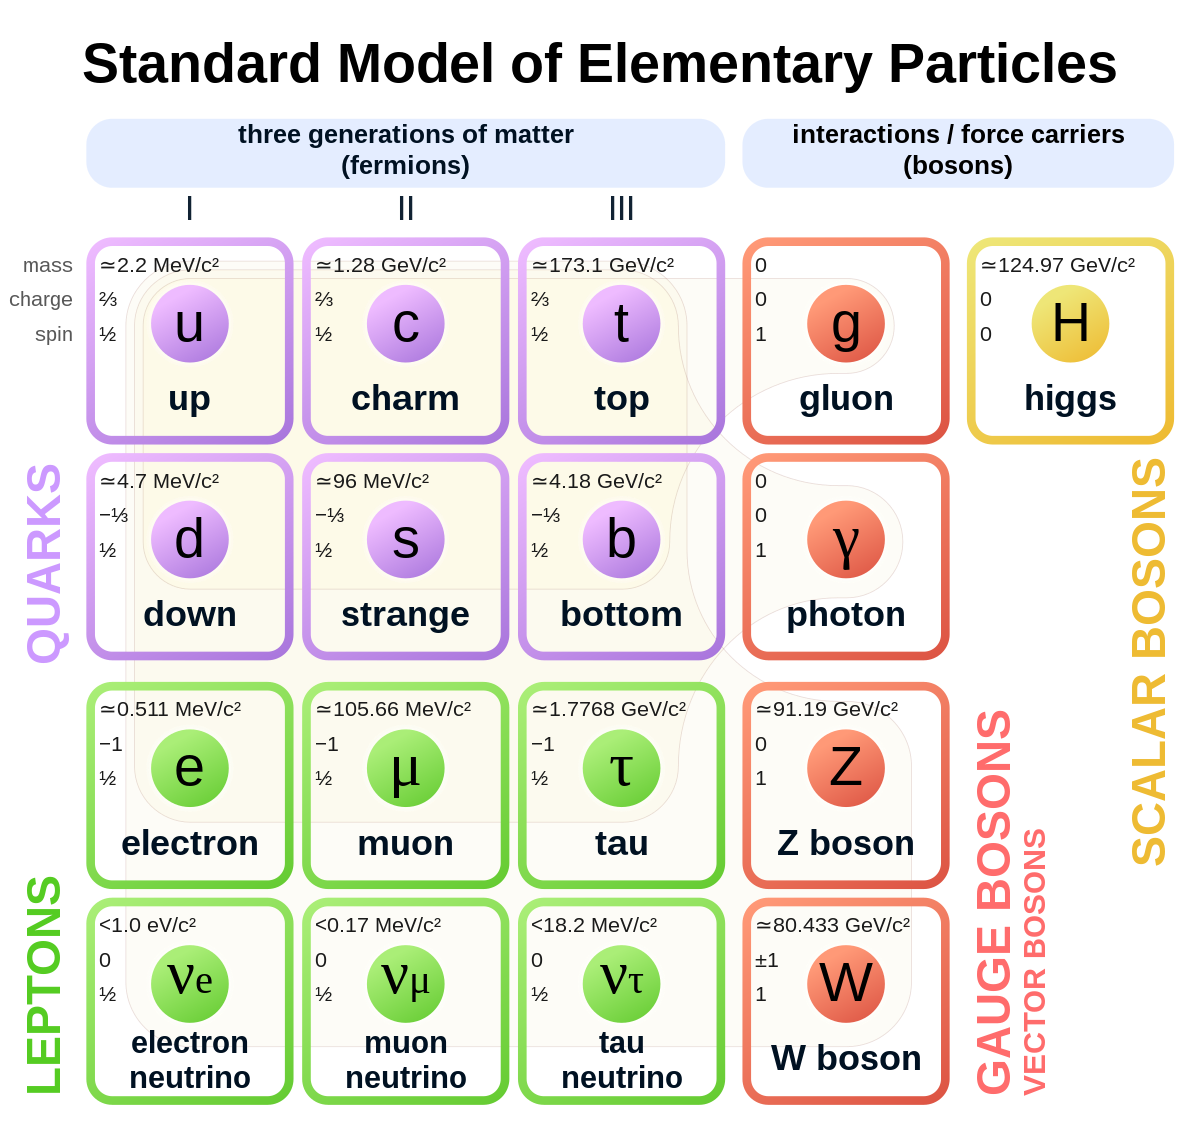
\includegraphics[width=\linewidth]{Figures/SM/Standard_Model_of_Elementary_Particles.svg.png}
    \caption{The standard model of elementary particles. Source \href{https://upload.wikimedia.org/wikipedia/commons/thumb/0/00/Standard_Model_of_Elementary_Particles.svg/1200px-Standard_Model_of_Elementary_Particles.svg.png}{here}. Accessed 07.10.22}
    \label{fig:smdiagram}
\end{figure}


\subsection*{Fermions}
The fermions are the building blocks of matter, and contain two types of particles, leptons and quarks. Together they form protons and neutrons,  atoms all around us.
Fermions, unlike bosons, are spin half particles, and are also the only particles to have anti particles. 


\subsubsection*{Quarks}
Quarks are fractional charge particles, with defined charge of either $2/3$ or $-1/3$. They are the building blocks of protons and neutrons


\subsection*{Bosons}


\section*{Limitations}
All though the standard model have had great success comparing with experiments,
there are still several problems not addressed by it. First and foremost, the standard model
as described above, does not and cannot explain gravity in a quantized way. There 
are models that try to address this problem, but they supplement the standard model,
and does not derrive it from it. 

